%\section{\SecAdvanceBulkjob} \label{sec:bulkjob}
%====================================================================================

\section{バルクジョブとは?} \label{sec:bulkjob}
\scalerm には、独立した実験を同時に複数実行できる「一括実行機能」、いわゆるバルクジョブ機能が備わっている。
この機能は、パラメタスイープ実験、初期値アンサンブル実験、
タイムスライス気候実験等を行うのに便利である。

バルクジョブ機能は、モデル本体(\verb|scale-rm|)の実行はもちろん、
地形・土地利用データ、初期値/境界値データの作成にも適用できる。
ただし、バルクジョブ機能による地形・土地利用データの作成は、地形コピー機能(第\ref{subsec:nest_topo}節を参照)を利用しない場合に限る。

以下の説明では、1のバルクジョブに含まれる独立した実行命令を「サブジョブ」と呼ぶこととする。
ここでは、3つの2段オンライン・ネスティング実験を例に説明する。
この3つの実験は、積分期間もしくは計算領域中心が異なる3つのサブジョブを想定している。
ファイル\verb|launch.conf|中の\namelist{PARAM_LAUNCHER}の\nmitem{NUM_DOMAIN, PRC_DOMAINS, CONF_FILES}(第\ref{subsubsec:launch}節参照)は、全ての設定で同じにする必要がある。
その他の設定(積分時間、使用するスキーム、1つのMPIプロセスあたりの格子数等)は、
サブジョブ間で異なっていても構わない。

\begin{figure}[t]
\begin{center}
  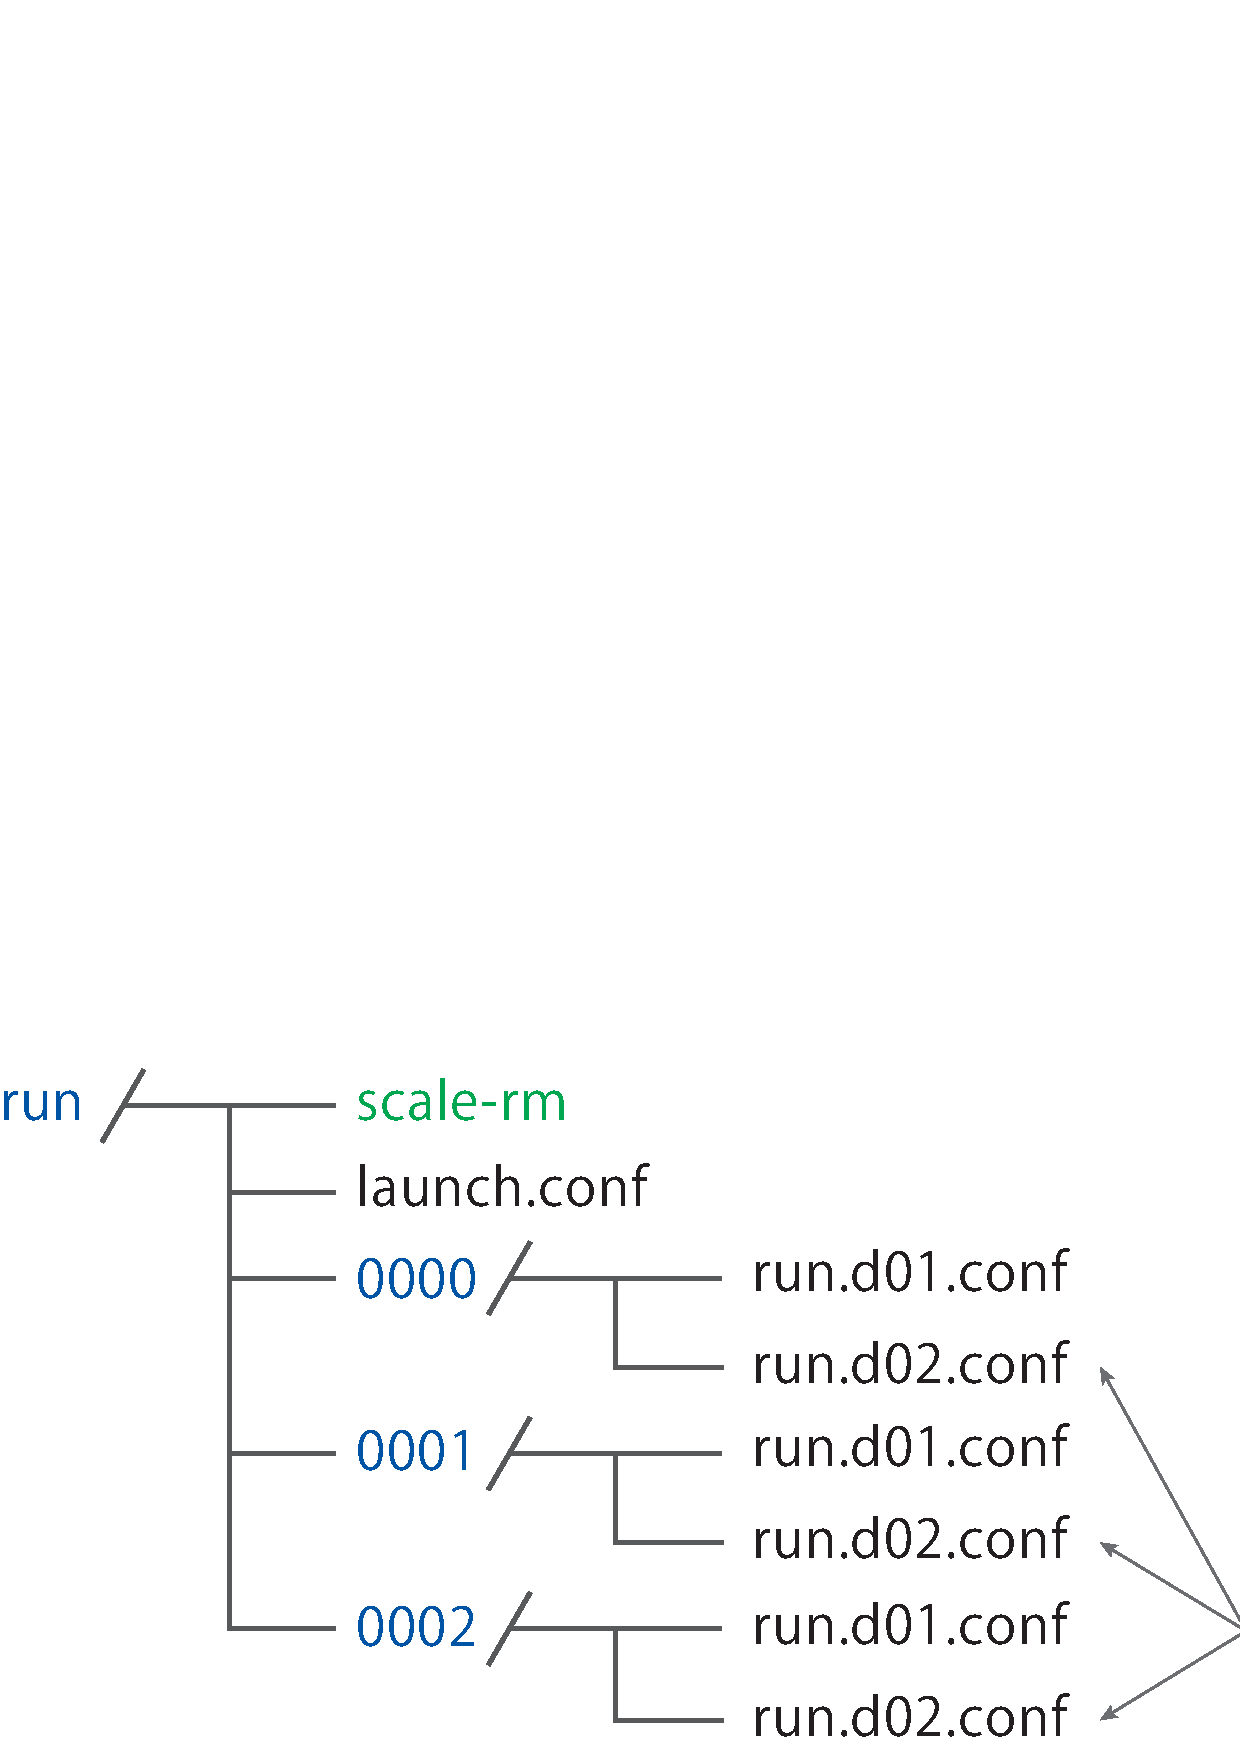
\includegraphics[width=0.6\hsize]{./../../figure/bulkjob_directory_structure.pdf}\\
  \caption{バルクジョブ機能を使って\texttt{scale-rm}を実行する場合のディレクトリ構造. 「0000」や「0001」といった数字は、ジョブ番号に対応するディレクトリ(ジョブディレクトリと呼ぶ)の名前である。各ジョブディレクトリの中には、サブジョブの実行に必要な全設定ファイルが用意されていなければならない。}
  \label{fig_bulkjob}
\end{center}
\end{figure}


\section{バルクジョブの設定}
バルクジョブ機能は、オンライン・ネスティングで利用した
MPIプロセスを分割・分配する機能を拡張したものである。
従って、ジョブの起動のために\verb|launch.conf|ファイルが必要になる。
オンライン・ネスティングとバルクジョブ機能を併用する場合も、
\verb|launch.conf|ファイルは1個だけ用意すれば良い。
そのような場合の例を、以下に示す。
\editboxtwo{
\verb|&PARAM_LAUNCHER|       & \\
\verb| NUM_BULKJOB = 3,|     & サブジョブの数\\
\verb| NUM_DOMAIN  = 2,|     & ネスティング領域の数\\
\verb| PRC_DOMAINS = 9, 36,|  & 各領域の全プロセス数\\
\verb| CONF_FILES  = run.d01.conf, run.d02.conf,| & 設定ファイル名\\
\verb| LOG_SPLIT   = .false.,| & MPI 分割に関するログを出力するか?\\
\verb| COLOR_REORDER = .true.,| & MPI 分割におけるプロセス番号の再割り当てを行うか?\\
\verb| FAILURE_PRC_MANAGE = .false.,| & 失敗したプロセスの管理機能を使用するか?\\
\verb| NUM_FAIL_TOLERANCE = 1, | & 失敗プロセスの許容数 \\
\verb| FREQ_FAIL_CHECK    = 5, | & DT ごとの FPM による調査頻度 \\
\verb|/| \\
}

サブジョブの数は \nmitem{NUM_BULKJOB} で指定します。
シングルドメインの実験 (ネスティングは使用しない) の場合は、\nmitem{NUM_DOMAIN} $=$ 1 を指定する。

ジョブディレクトリ名は4桁の数字で、デフォルトでは0から始まるジョブIDに対応します。
\nmitem{BULKJOB_START_DIRNUM}を指定することで、開始番号を変更することができます。

デフォルトでは、サブジョブの設定ファイル (init.conf、run.conf など) 中のファイル名には、ジョブのディレクトリ名が含まれていなければなりません(例:0000/history.nc)。
\nmitem{ADDD_BULJJOB_PATH}を \verb|.true.| に指定すると、絶対パス以外のすべてのファイル名にジョブディレクトリ名が追加されます。

利用する計算機においてサブジョブを一度に実行できるだけのリソースがない場合は、サブジョブを複数のグループに分けることができます。
一度に実行されるサブジョブの数は \nmitem{NUM_BULKJOB} / \nmitem{NUM_ITERATION_BULK} 個になります。


他の設定は、第\ref{subsubsec:launch}節における設定と同様である。



\section{失敗プロセスの管理}
\scalerm のバルクジョブシステムでは、失敗プロセスの管理(failure process management ; FPM)ツールが使用できる。
FPM は、ある調査周期でジョブグループを監視する。
いくつかのジョブが不幸にも異常終了した場合でも、失敗したジョブ数が制限値に達するまでは他のジョブを終了させない。
\nmitem{FAILURE_PRC_MANAGE} は FPM ツールを用いるためのスイッチである。
\nmitem{NUM_FAIL_TOLERANCE} と \nmitem{FREQ_FAIL_CHECK} はそれぞれ、失敗したジョブの制限値と失敗したジョブを調べる間隔を設定するパラメータである。
FPM ツールの現版では、単一領域に対してのみ使用でき、オンライン・ネスティング計算での完全なシステムには対応していない。
オンライン・ネスティング計算においても FPM ツールを使用したい場合は、\nmitem{NUM_FAIL_TOLERANCE}を全ジョブ数と同じにしなければならない。


\section{バルクジョブのための準備}
バルクジョブの実行にあたり、サブジョブの数だけ
ディレクトリ(ジョブディレクトリと呼ぶ)を用意する必要がある。
図\ref{fig_bulkjob}において、ジョブディレクトリは\verb|0000/  0001/  0002/|に対応する。
ディレクトリ名には、ゼロから始まる4桁の数字が付けられる。
各ジョブディレクトリには、実験に必要な全てのファイル
(設定ファイル、入力ファイル、出力用ディレクトリ等)を用意しなければならない。
%
設定ファイルに指定されているディレクトリやファイルのパスが、
以下で説明するように適切に設定されているか注意する必要がある。
以下は、ジョブ\verb|0000|の\verb|run.d01.conf|の抜粋である。\\
\editbox{
\verb|&PARAM_IO| \\
\verb| IO_LOG_BASENAME = "0000/LOG_d01",| \\
\verb|/| \\
 \\
\verb|&PARAM_RESTART| \\
\verb| RESTART_OUTPUT       = .true.,| \\
\verb| RESTART_OUT_BASENAME = "0000/restart_d01",| \\
\verb| RESTART_IN_BASENAME  = "../init/0000/init_d01_00013046400.000",| \\
\verb|/| \\
 \\
\verb|&PARAM_TOPOGRAPHY| \\
\verb| TOPOGRAPHY_IN_BASENAME = "../pp/0000/topo_d01",| \\
\verb|/| \\
 \\
\verb|&PARAM_LANDUSE| \\
\verb| LANDUSE_IN_BASENAME = "../pp/0000/landuse_d01",| \\
\verb|/| \\
 \\
\verb|&PARAM_ATMOS_BOUNDARY| \\
\verb| ~ ... ~             | \\
\verb| ATMOS_BOUNDARY_IN_BASENAME    = "../init/0000/boundary_d01",| \\
\verb| ~ ... ~             | \\
\verb|/                    | \\
 \\
\verb|&PARAM_FILE_HISTORY| \\
\verb| FILE_HISTORY_DEFAULT_BASENAME  = "0000/history_d01",| \\
\verb| ~ ... ~           | \\
\verb|/| \\
}

図\ref{fig_bulkjob}に示すように、
ジョブディレクトリは実行バイナリと同じディレクトリの階層にある。
つまり、設定ファイルは各ジョブディレクトリの下にあるが、
入力ファイルや出力先のディレクトリは、実行バイナリの位置から見た相対パスを記述する必要がある。
従って、ジョブ0000番の実験に対する出力用ディレクトリは\verb|0000/|であり、
出力ファイル名は\verb|0000/***|となる。
{\color{blue}{ジョブディレクトリ名を付け忘れてファイル名を全実験で同じにしてしまうと、同じファイルに出力を行うためデータが消失することに注意されたい。}}

\section{バルクジョブの実行}
バルクジョブの実行時には、以下のようにMPIプロセスの総数を指定する。
\begin{verbatim}
 $ mpirun  -n  135  ./scale-rm  launch.conf
\end{verbatim}
この例では、1 サブジョブあたりが使用するプロセス数は 45 ($=9 + 36$)であり、
3つのジョブで使用するプロセスの総数は 135 である。
MPI のプロセス分割に関する情報を与えるメッセージは、LOG ファイルの中の \scalelib のロゴの後に書き込まれる。下記は、ドメイン1のプロセス0からのログの出力例である。\\
\msgboxtwo{
\verb| +++++ start making Cartesian topology|  & \\
\verb| *** UNIVERSAL_COMM_WORLD        :        0| &; 実行環境によって値が異なる\\
\verb| *** total process [UNIVERSAL]   :      135| &\\
\verb| *** my process ID [UNIVERSAL]   :       36| &\\
\verb| *** master rank?  [UNIVERSAL]   :        F| &\\
\verb| *** GLOBAL_COMM_WORLD           :        3| &; 実行環境によって値が異なる \\
\verb| *** total process [GLOBAL]      :       45| &\\
\verb| *** my process ID [GLOBAL]      :       36| &\\
\verb| *** master rank?  [GLOBAL]      :        F| &\\
\verb| *** LOCAL_COMM_WORLD            :        4| &; 実行環境によって値が異なる \\
\verb| *** total process [LOCAL]       :        9| &\\
\verb| *** my process ID [LOCAL]       :        0| &\\
\verb| *** master rank?  [LOCAL]       :        T| &\\
\verb| *** ABORT_COMM_WORLD            :        0| &\\
\verb| *** master rank ID [each world] :        0| &\\
&\\
}
\verb|[LOCAL]|と表記されている項目は、ドメイン内のプロセスグループに関する情報である。
また、\verb|[GLOBAL]|と表記されている項目はネスティンググループ、
\verb|[UNIVERSAL]|と表記されている項目はジョブグループに関する情報である。
\verb|LOCAL|グループは\verb|GLOBAL|グループに包含され、
さらに\verb|GLOBAL|グループは\verb|UNIVERSAL|グループに包含される。
\verb|total process|は各グループ内の全プロセス数、\verb|my process ID|はあるグループで見た時のプロセス番号を表す。

この例では、\verb|total process [UNIVERSAL]|は135であるので、全体で135のプロセスが起動したことが確認できる。
また、\verb|total process [GLOBAL]|は45であるので、
1サブジョブあたり45プロセスを使用したことが分かる。
この例ではドメイン1に対するLOGメッセージであるため、
\verb|total process [LOCAL]|が9と表記されていることは正しい。
もしドメイン2のLOGメッセージを確認した場合、これは 36 である。
LOGファイルやヒストリファイルの番号に対応するプロセス番号は、\verb|my process ID [UNIVERSAL]|である。
異常終了時にも、この表記法に従ってメッセージが出力される。
そのため、この表記法を理解していれば、大量のサブジョブを実行している時にどのプロセスでエラーが発生したか即座に判断できる。

%%%%%%%%%%%%%%%%%%%%%%%%%%%%%%%%%%%%%%%%%%%%%%%%%%%%%%%%%%%%%%%%%%%%%%%%%%%%%%%%%%%%%%
